\chapter{색 표현, 강입자, 그리고 가둠}

\paragraph{짧은 도입부.}
군론으로 돌아가기 전에 염치 불고하고 짧게 홍보 하나만 하겠습니다. \emph{블랙홀 전쟁}은 블랙홀이 양자 정보를 파괴하는지를 두고 스티븐 호킹과 오랫동안 논쟁한 이야기를 담고 있습니다. 이 책에는 이론물리학자 특유의 잔인함도 기록되어 있습니다. 슈뢰딩거의 고양이뿐 아니라 서스킨드의 물고기와 그 불운한 변기행까지 말입니다. 이 책무를 마쳤으니 앨리스와 밥으로 돌아갑시다. 밥이 여전히 앨리스에게 군론을 배우게 하고 있으니, 앨리스는 아직도 고생 중입니다.

\lectureoverview{대칭은 상태에 작용할 때 물리적 의미를 갖습니다. 먼저 회전을 이용해 표현과 생성자를 소개한 다음, 색 \(SU(3)\)에 대해서도 같은 구성을 살펴보겠습니다. 색 표현들이 결합해 강입자를 이루며, 그 동역학은 고립된 색이 관측되지 않는 이유를 설명합니다.}

\section{군과 군이 작용하는 대상}

대칭을 논할 때는 두 가지 개념이 있습니다. 첫째는 곱셈 법칙과 항등원, 역원을 갖는 연산들의 모임인 추상군입니다. 둘째는 그 연산들이 작용하는 대상입니다. 두 개념은 구분할 수 있지만, 물리학에서는 서로 떼어 놓을 수 없습니다. 대칭이 중요한 까닭은 물리적 상태, 장, 좌표 또는 관측량을 변환하기 때문입니다.

\begin{classroomqa}
\audiencequestion{군을 추상적인 곱셈표로 설명하기도 하고 물리적 대상에 작용하는 행렬로 설명하기도 했습니다. 이 두 부분을 분리할 수 있습니까?
\lecturetimestamp{00:01:58}}
\lecturerresponse{서로 다른 기술 수준이지만 완전히 연결되어 있습니다. 회전은 무엇을 회전시키는지 정하기 전에도 추상적 연산으로 존재합니다. 그런 다음 물리학에서는 같은 연산이 특정 계와 관련된 상태와 양에 어떻게 작용하는지 묻습니다. 행렬은 추상적인 곱셈 법칙을 보존하면서 그 작용을 구체적으로 나타냅니다.}
\end{classroomqa}

공간 회전이 가장 명료한 예입니다. 고전적으로 같은 회전은 입자의 좌표, 자석의 방향 또는 다른 벡터에 작용할 수 있습니다. 양자역학에서 상태는 선형 벡터 공간에 있으므로, 회전은 그 공간에 작용하는 선형 연산자로 표현됩니다. 추상군 원소를 \(g\), 그 행렬 표현을 \(D(g)\)라 하면, 일관성을 위해 다음이 성립해야 합니다.
\begin{equation}
D(g_1g_2)=D(g_1)D(g_2),
\qquad
D(e)=\boldsymbol 1.
\end{equation}
행렬이 추상적인 연산과 같은 모양일 필요는 없지만, 행렬의 곱셈은 군의 곱셈을 재현해야 합니다.
\editorialnote{준동형 방정식은 원문에서 말로 설명한 군 곱셈과 행렬 곱셈 사이의 대응을 명시적으로 나타냅니다.}

행렬의 차원은 추상군만으로 정해지는 것이 아니라 상태 공간으로 정해집니다. 전자 하나의 스핀만 고려하면 서로 직교하는 두 가지 가능성, 즉 스핀 위와 스핀 아래가 있고, 상태는 두 성분 열벡터입니다. 따라서 회전은 \(2\times2\) 행렬로 작용합니다. 스핀 1/2인 두 대상에는 네 가지 기저 상태가 있습니다.
\begin{equation}
\ket{\uparrow\uparrow},\qquad
\ket{\uparrow\downarrow},\qquad
\ket{\downarrow\uparrow},\qquad
\ket{\downarrow\downarrow},
\end{equation}
결합된 공간에서 유도되는 작용은 4차원입니다.

익숙한 순서는 다음과 같습니다.
\begin{equation}
\begin{array}{c|c|c}
\text{spin} & \text{number of states} & \text{matrix dimension}\\
\hline
0 & 1 & 1\times1\\
\frac12 & 2 & 2\times2\\
1 & 3 & 3\times3\\
\frac32 & 4 & 4\times4
\end{array}
\end{equation}
스핀 0 상태는 자명 표현을 이룹니다. 모든 회전이 이 상태를 그대로 둡니다. 1×1 행렬은 그저 \(1\)입니다. 스핀 1 상태에는 세 성분이 있으며, 그 회전 행렬은 익숙한 3차원 벡터 회전 행렬입니다. 더 일반적으로 스핀 \(j\)에는 \(2j+1\)개의 상태가 있습니다.

표현은 무한 차원일 수도 있습니다. 전자의 스핀만이 아니라 전체 궤도 운동을 기술하면, 상태에는 위치마다, 또는 동등하게 운동량마다 진폭이 있습니다. 그러면 회전 연산자는 무한 차원 파동함수 공간에 작용합니다. 따라서 하나의 추상 회전군이 자명 표현, 2차원 표현, 3차원 표현, 무한 차원 표현을 모두 가질 수 있습니다. 논의가 스핀에서 색으로 옮겨갈 때 이 사실을 다시 활용하겠습니다.

\section{스핀 회전이 특수 유니터리인 이유}

이제 전자 하나의 스핀으로 돌아가 궤도 운동은 제외합시다. 회전은 \(2\times2\) 유니터리 행렬 \(U\)로 표현됩니다.
\begin{equation}
U^\dagger U=\boldsymbol 1,
\qquad
U^{-1}=U^\dagger.
\label{eq:l4-unitarity}
\end{equation}
역변환은 회전을 되돌려야 하며, 유니터리성은 노름과 따라서 모든 확률을 보존합니다.

일반적인 \(2\times2\) 복소 행렬에는 복소 성분이 네 개, 즉 실수 매개변수가 여덟 개 있습니다. 식~\eqref{eq:l4-unitarity}은 서로 독립인 실수 조건 네 개를 부과하므로 매개변수 네 개가 남습니다. 보통의 공간 회전에는 매개변수가 세 개뿐입니다. 두 개는 회전축을 정하고 하나는 각도를 정합니다. 따라서 유니터리 행렬에는 위상이 하나 더 들어 있습니다. 추가 제약은 다음과 같습니다.
\begin{equation}
\det U=1.
\label{eq:l4-det-one}
\end{equation}
그러면 매개변수 개수는 다음과 같습니다.
\begin{equation}
8-4-1=3.
\end{equation}

행렬식이 1이라는 조건은 곱셈에 대해 보존된다.
\begin{equation}
\det(AB)=\det A\,\det B.
\end{equation}
행렬식이 각각 1인 두 행렬의 곱도 같은 조건을 만족하기 때문이다. 이 조건은 유니터리성과도 양립한다. ~\eqref{eq:l4-unitarity}의 양변에 행렬식을 취하면
\begin{equation}
1=\det(U^\dagger U)
=\det(U^\dagger)\det U
=(\det U)^*\det U.
\end{equation}
따라서 유니터리 행렬의 행렬식은 복소평면의 단위원 위에 놓인다.
\begin{equation}
\det U=e^{i\phi}.
\end{equation}

\begin{classroomqa}
\audiencequestion{유니터리성은 행렬식이 실수여야 한다는 뜻인가요?
\lecturetimestamp{00:12:10}}
\lecturerresponse{아닙니다. 유니터리성이 요구하는 것은 절댓값이 1이라는 조건뿐입니다. 행렬식은 임의의 순수 위상 \(e^{i\phi}\)일 수 있습니다. 2차원 행렬에서는 \(U\)에 \(e^{-i\phi/2}\)를 곱해 공통 위상을 없애면 행렬식이 1인 행렬을 얻습니다.}
\end{classroomqa}

실제로,
\begin{equation}
V=e^{-i\phi/2}U,
\end{equation}
이라면 \(V\)는 여전히 유니터리이고,
\begin{equation}
\det V=e^{-i\phi}\det U=1.
\end{equation}
행렬식이 1인 유니터리 행렬들은 \(SU(2)\)을 이룹니다.

여기에는 한 가지 세밀한 점이 있습니다. \(SU(2)\)가 3차원 공간의 회전군이라고만 말하고 싶겠지만, 대응은 두 대 일입니다. 행렬 \(U\)와 \(-U\)는 스피너에 서로 다르게 작용하지만, 보통의 벡터를 같은 회전으로 변환합니다. 따라서
\begin{equation}
SU(2)/\{\boldsymbol 1,-\boldsymbol 1\}\simeq SO(3).
\end{equation}
현재 논의에서는 국소적인 곱셈 구조와 세 생성자가 중요하지만, 이중 덮개 구조는 스핀 1/2 회전이 두 값을 갖는 이유를 설명합니다.

\section{무한소 변환과 그 생성자}

유한 회전은 아주 작은 회전들을 여러 번 적용해 만들 수 있습니다. 항등원에 가까운 군 원소를 무한소 원소라고 하며, 연결군에서는 모든 무한소 방향을 알면 반복적인 곱셈으로 유한 변환을 재구성하기에 충분합니다. 물리학에서 더 중요한 점은 이러한 무한소 변환을 생성하는 연산자가 대칭에 대응하는 보존량이라는 사실입니다.

항등원에 가까운 원소를 다음과 같이 씁니다.
\begin{equation}
U=\boldsymbol 1+i\epsilon T,
\qquad |\epsilon|\ll1.
\label{eq:l4-infinitesimal-u}
\end{equation}
\(i\) 인자는 편리한 약속입니다. 이를 유니터리 조건에 대입하고 \(\epsilon^2\) 차수 항을 버리면
\begin{align}
(\boldsymbol 1+i\epsilon T)
(\boldsymbol 1-i\epsilon T^\dagger)&=\boldsymbol 1,
\\
i\epsilon(T-T^\dagger)&=0,
\\
T&=T^\dagger.
\label{eq:l4-hermitian-generator}
\end{align}
양자역학적 관측량이어야 하는 생성자는 에르미트 연산자입니다.

\begin{figure}[htbp]\centering
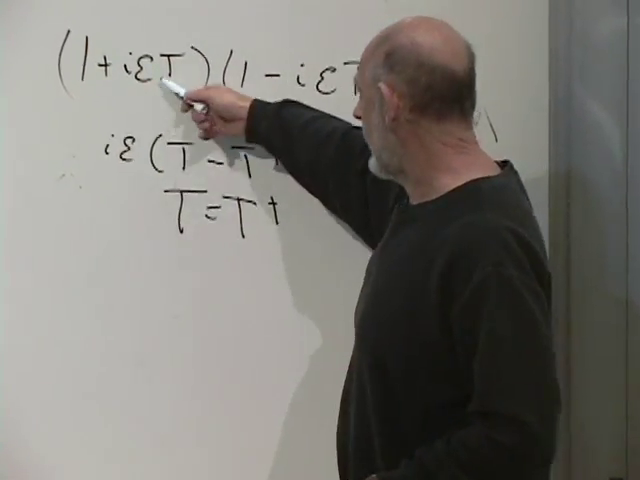
\includegraphics[width=0.62\textwidth]{lecture_04_figure_03.png}\caption{항등원에 가까운 유니터리 조건을 계산하면 \(T=T^\dagger\)이 됩니다.}\lectureframe{00:23:28}\end{figure}

공간 회전에는 독립적인 무한소 회전축이 세 개이므로 선형 독립인 생성자가 세 개 있습니다. 임의의 방향을 축으로 하는 작은 회전은 \(x\), \(y\), \(z\) 축을 중심으로 한 작은 회전들을 조합해 이룹니다. 이에 대응하는 생성자는 각운동량 연산자 \(J_x,J_y,J_z\)입니다. 이들의 교환자는 회전의 비가환성을 나타냅니다.
\begin{equation}
[J_i,J_j]=i\epsilon_{ijk}J_k.
\label{eq:l4-angular-momentum-algebra}
\end{equation}
무한소 회전을 반복하면 유한 회전이 만들어집니다.

유니터리성은 사용했지만 행렬식이 1이라는 조건은 아직 사용하지 않았습니다. 임의의 작은 행렬 \(m\)에 대해
\begin{equation}
\det(\boldsymbol 1+\epsilon m)
=1+\epsilon\,\operatorname{tr}m+O(\epsilon^2).
\label{eq:l4-det-expansion}
\end{equation}

\begin{figure}[htbp]\centering
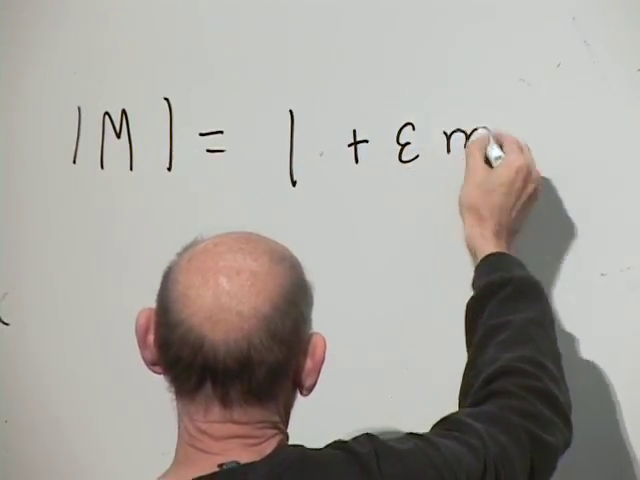
\includegraphics[width=0.62\textwidth]{lecture_04_figure_02.png}\caption{칠판에 적힌 행렬식의 1차 전개.}\lectureframe{00:21:51}\end{figure}

~\eqref{eq:l4-det-expansion}을 ~\eqref{eq:l4-infinitesimal-u}에 적용하면,
\begin{equation}
\det U
=1+i\epsilon\,\operatorname{tr}T+O(\epsilon^2).
\end{equation}
따라서 특수 유니터리 조건은 다음을 요구한다.
\begin{equation}
\operatorname{tr}T=0.
\label{eq:l4-traceless-generator}
\end{equation}
\(SU(2)\)의 생성자는 정확히 자취가 없는 에르미트 \(2\times2\) 행렬이다. 이 벡터 공간은 3차원이다. 파울리 행렬이 표준 기저를 이룬다.
\begin{equation}
\begin{aligned}
\sigma_x&=
\begin{pmatrix}0&1\\1&0\end{pmatrix},
&
\sigma_y&=
\begin{pmatrix}0&-i\\i&0\end{pmatrix},
\\[0.4em]
\sigma_z&=
\begin{pmatrix}1&0\\0&-1\end{pmatrix}.
\end{aligned}
\end{equation}
스핀 1/2 표현에서는 \(J_i=\sigma_i/2\)로 둘 수 있으므로, \(\hat{\boldsymbol n}\)을 축으로 \(\theta\)만큼 회전하는 유한 회전은
\begin{equation}
U(\hat{\boldsymbol n},\theta)
=\exp\!\left(-i\theta\,
\hat{\boldsymbol n}\cdot\boldsymbol\sigma/2\right).
\end{equation}
\editorialnote{유한 지수식은 무한소 생성자에 관한 논의를 표준적으로 마무리한다. 원문은 이 식을 명시적으로 쓰기보다 작은 회전을 반복하는 방식을 강조한다.}

\begin{classroomqa}
\audiencequestion{서로 독립인 자취 없는 에르미트 \(2\times2\) 행렬이 세 개라는 뜻인가요?
\lecturetimestamp{00:24:07}}
\lecturerresponse{그렇습니다. 파울리 행렬 세 개입니다. \(3\times3\) 특수 유니터리 행렬의 경우 이에 대응하는 개수는 여덟이며, 표준 기저는 겔만 행렬 여덟 개로 주어집니다.}
\end{classroomqa}

\begin{classroomqa}
\audiencequestion{그 여덟은 팔중도와 글루온 여덟 개에서 말하는 ``여덟''과 같은 건가요?
\lecturetimestamp{00:24:43}}
\lecturerresponse{수학적으로는 같은 유형의 \(SU(3)\) 표현론이지만, 어떤 \(SU(3)\) 대칭이 작용하는지 분명히 해야 합니다. 역사적인 팔중도 맛깔 대칭은 색 \(SU(3)\)이 아닙니다. 글루온 여덟 개는 색 \(SU(3)\)의 수반 표현에 속합니다.}
\end{classroomqa}

\section{SU(2)에서 색 SU(3)로}

이제 행렬을 \(2\times2\)에서 \(3\times3\)로 키워 봅시다. 일반적인 복소 \(3\times3\) 행렬에는 복소 성분이 아홉 개, 즉 실수 매개변수가 열여덟 개 있습니다. 조건 \(U^\dagger U=\boldsymbol 1\)은 실수 제약 아홉 개를 부과하고, \(\det U=1\)은 하나를 더 줄입니다. 따라서
\begin{equation}
18-9-1=8.
\end{equation}
독립적인 무한소 방향은 여덟 개이고 자취 없는 에르미트 생성자도 여덟 개입니다. \(SU(2)\)와 달리 이 군은 보통의 3차원 공간에서 회전군이 아닙니다. 색에 작용하는 내부 대칭입니다.

이 표현들을 쿼크에 적용하기 전에 합성 표현이 어떻게 생기는지 떠올려 봅시다. 스핀 1/2인 두 계를 포개고 궤도 운동은 무시합시다. 곱 상태는 네 개지만, 회전은 이 네 상태 전체를 기약적으로 섞지는 않습니다. 세 조합은 스핀 1처럼 변환합니다.
\begin{align}
\ket{1,1}&=\ket{\uparrow\uparrow},\\
\ket{1,0}&=\frac{1}{\sqrt2}
(\ket{\uparrow\downarrow}+\ket{\downarrow\uparrow}),\\
\ket{1,-1}&=\ket{\downarrow\downarrow},
\end{align}
네 번째 조합은 스핀 0처럼 변환합니다.
\begin{equation}
\ket{0,0}=\frac{1}{\sqrt2}
(\ket{\uparrow\downarrow}-\ket{\downarrow\uparrow}).
\end{equation}
따라서
\begin{equation}
\boldsymbol 2\otimes\boldsymbol 2
=\boldsymbol 3\oplus\boldsymbol 1.
\label{eq:l4-two-spin-decomposition}
\end{equation}
정렬된 상태가 삼중항의 \(m=\pm1\) 성분을 이루고, 대칭인 영 투영 상태가 삼중항을 완성하며, 반대칭 조합은 단일항입니다. 이것이 각운동량을 더하는 일반적인 원리이자 색 표현을 결합하는 원리입니다.

같은 단일항--삼중항 구분은 스핀 1/2 자유도 두 개를 결합할 때마다 나타납니다. 원자 수소에서는 전자와 양성자의 스핀이 초미세 단일항 및 삼중항 상태를 이룹니다. 오르토 수소와 파라 수소에서도 \(H_2\) 분자 안에 있는 두 양성자의 핵스핀에 같은 표현론이 적용됩니다.
\editorialnote{원문은 원자 수소의 양성자--전자 스핀을 언급하면서 ``오르토 및 파라 수소''라는 표현을 사용합니다. 수학적 분해는 맞습니다. 여기서는 정확성을 위해 분자 상태와 원자 상태의 명칭을 구분했습니다.}

\subsection{삼중항과 반삼중항}

쿼크 하나에는 세 가지 색 진폭이 있습니다. 선택한 기저에서 다음과 같이 씁니다.
\begin{equation}
q=
\begin{pmatrix}
q_r\\q_g\\q_b
\end{pmatrix},
\qquad
q'=Uq,
\qquad U\in SU(3).
\label{eq:l4-quark-triplet}
\end{equation}
세 성분은 쿼크 하나의 상태 진폭일 수도 있고, 빨강·초록·파랑 쿼크를 생성하는 세 장 연산자일 수도 있습니다. 군은 세 성분을 서로 섞습니다. 처음에 빨강인 상태는 일반적으로 색 변환 후 빨강·초록·파랑의 중첩 상태가 됩니다. 이 기본 3차원 표현을 \(\boldsymbol 3\)이라고 합니다.

반쿼크에는 쿼크 표현의 복소켤레를 통해 군이 작용합니다. 식~\eqref{eq:l4-quark-triplet}의 복소켤레를 취하면
\begin{equation}
\bar q'=U^*\bar q.
\end{equation}
이 표현을 \(\bar{\boldsymbol 3}\)라고 표기합니다. \(U(1)\)의 유비는 명확합니다. 전자장이 \(e^{i\theta}\)를 얻으면 양전자장은 \(e^{-i\theta}\)를 얻습니다. 쿼크와 반쿼크의 색 변환은 이 켤레 짝짓기의 비가환 버전입니다.

항등원 가까이에서 다음과 같다면
\begin{equation}
U=\boldsymbol 1+i\epsilon T,
\end{equation}
다음이 성립합니다.
\begin{equation}
U^*=\boldsymbol 1-i\epsilon T^*.
\end{equation}
따라서 반삼중항 생성자는 \(-T^*\), 즉 부호가 반대인 켤레입니다. 이것이 반쿼크가 반대 색전하를 가진다는 말의 정확한 의미입니다.

\begin{classroomqa}
\audiencequestion{\(SU(2)\)의 경우 복소켤레 표현은 어떻게 되나요?
\lecturetimestamp{00:36:19}}
\lecturerresponse{\(SU(2)\)의 이중항은 특별한 경우입니다. 반대칭 엡실론 텐서를 포함하는 고정된 기저 변환을 거치면 복소켤레 표현이 원래의 이중항과 동등합니다. \(SU(3)\)에서는 \(\boldsymbol 3\)와 \(\bar{\boldsymbol 3}\)가 실제로 서로 동등하지 않은 표현입니다.}
\end{classroomqa}
\editorialnote{\(SU(2)\) 기본 표현의 수학적으로 정확한 용어는 실수 표현이 아니라 유사실수 표현입니다. 답변은 원문의 의도된 구분을 유지하면서 용어를 바로잡았습니다.}

\section{색 표현의 결합}

기호 \(\otimes\)는 그 옆에 적힌 수를 보통의 방식으로 곱한다는 뜻이 아닙니다. 두 상태 공간을 결합한다는 뜻입니다. 그렇게 얻은 텐서곱 공간은 군 작용 아래 서로 섞이지 않는 부분들로 다시 분해됩니다.

\subsection{\texorpdfstring{\(\boldsymbol 3\otimes\boldsymbol 3\)}{두 쿼크: 33 x }}

쿼크 두 개에는 아홉 가지 색 기저 상태가 있습니다. 빨강--빨강, 빨강--초록, 빨강--파랑과 나머지 여섯 가지 순서쌍입니다. 두 색 지표를 대칭 부분과 반대칭 부분으로 나눠 봅시다. 대칭 부분에는 독립 성분이 여섯 개, 반대칭 부분에는 세 개 있습니다. \(SU(3)\)에서는
\begin{equation}
\boldsymbol 3\otimes\boldsymbol 3
=\boldsymbol 6\oplus\bar{\boldsymbol 3}.
\label{eq:l4-three-times-three}
\end{equation}

\begin{figure}[htbp]\centering
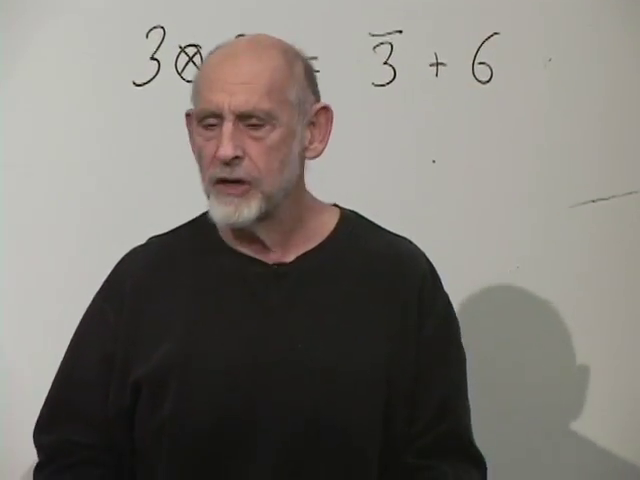
\includegraphics[width=0.68\textwidth]{lecture_04_figure_04.png}\caption{쿼크 두 개의 곱이 반삼중항과 육중항으로 분해됩니다.}\lectureframe{00:39:33}\end{figure}

반삼중항은 두 쿼크 지표를 불변 엡실론 텐서와 수축해 명시적으로 나타낼 수 있습니다.
\begin{equation}
(qq)^k_{\bar 3}
=\frac{1}{\sqrt2}\epsilon^{kij}q_iq_j.
\end{equation}
이 대상은 성분 세 개를 가지며 반쿼크처럼 변환합니다. 대칭 조합 여섯 개는 육중항을 이룹니다. 쿼크 두 개가 동역학적으로 반쿼크가 된다는 뜻이 아닙니다. 색 파동함수의 한 부분이 반쿼크와 같은 변환 법칙을 따른다는 뜻입니다.

\subsection{\texorpdfstring{\(\boldsymbol 3\otimes\bar{\boldsymbol 3}\)}{쿼크와 반쿼크: 3 x 반-3}}

쿼크--반쿼크 색 상태는 \(3\times3\) 행렬 \(M_i{}^j=q_i\bar q^j\)로 볼 수 있습니다. 모든 행렬은 자취 부분과 자취 없는 부분으로 유일하게 분해됩니다.
\begin{equation}
M=\frac{\operatorname{tr}M}{3}\boldsymbol 1
+\left(M-\frac{\operatorname{tr}M}{3}\boldsymbol 1\right).
\end{equation}
자취 부분은 불변 성분 하나이고, 자취 없는 부분에는 성분 여덟 개가 있습니다. 따라서
\begin{equation}
\boldsymbol 3\otimes\bar{\boldsymbol 3}
=\boldsymbol 1\oplus\boldsymbol 8.
\label{eq:l4-three-times-threebar}
\end{equation}
정규화 상수를 제외하면 단일항은 다음과 같습니다.
\begin{equation}
\ket{1}_{q\bar q}
=\frac{1}{\sqrt3}
(\ket{r\bar r}+\ket{g\bar g}+\ket{b\bar b}).
\end{equation}
불변이므로 다른 상태로 회전해 갈 수 없습니다. 나머지 여덟 선형 조합은 서로 섞입니다. 이들은 생성자 여덟 개가 변환하는 것과 같은 표현인 수반 표현을 이룹니다.

\subsection{세 쿼크}

세 번째 쿼크를 ~\eqref{eq:l4-three-times-three}와 결합하면 반삼중항 분기에서 다음을 얻는다.
\begin{equation}
\bar{\boldsymbol 3}\otimes\boldsymbol 3
=\boldsymbol 1\oplus\boldsymbol 8,
\end{equation}
따라서 세 쿼크의 곱에는 단일항이 포함된다. 전체 분해는 다음과 같다.
\begin{equation}
\boldsymbol 3\otimes\boldsymbol 3\otimes\boldsymbol 3
=\boldsymbol 1\oplus\boldsymbol 8\oplus\boldsymbol 8
\oplus\boldsymbol{10}.
\label{eq:l4-three-quark-full}
\end{equation}
색 단일항은 완전히 반대칭인 빨강--초록--파랑 조합이다.
\begin{equation}
\ket{1}_{qqq}
=\frac{1}{\sqrt6}\epsilon^{ijk}\ket{q_iq_jq_k}.
\label{eq:l4-baryon-singlet}
\end{equation}
\(\epsilon^{ijk}\)는 두 지수가 같을 때마다 0이므로, 0이 아닌 모든 항에는 빨강, 초록, 파랑 쿼크가 하나씩 들어가며, 두 지수를 서로 바꾸면 부호가 바뀐다.

\begin{classroomqa}
\audiencequestion{단일항이 아닌 조합은 단지 일어날 확률이 낮아서 확률을 무시해도 되나요?
\lecturetimestamp{00:46:02}}
\lecturerresponse{아닙니다. 문제는 확률이 아니라 에너지입니다. 고립된 비단일항은 색장을 무한히 먼 거리까지 끌고 가며, 가둠 영역에서는 무한한 에너지가 필요합니다. 이 주장의 배경이 되는 동역학은 아래에서 다루겠습니다.}
\end{classroomqa}

\subsection{글루온 팔중항}

글루온 장은 식~\eqref{eq:l4-three-times-threebar}의 팔중항처럼 변환합니다. 색과 관련해서는 삼중항 지표 하나와 반삼중항 지표 하나를 가지며, 단일항 자취 성분은 제거되어 있습니다. 개략적으로 쓰면
\begin{equation}
q\sim\boldsymbol 3,
\qquad
\bar q\sim\bar{\boldsymbol 3},
\qquad
G\sim\boldsymbol 8.
\end{equation}
이 기호들은 변환 법칙을 나타냅니다. 입자가 문자 그대로 정수 3이나 8과 같다는 뜻은 아닙니다.

아홉 번째 쿼크--반쿼크 색 조합은 항등행렬에 비례하며 단일항이므로 팔중항과 섞이지 않습니다. 그러므로 이를 제외해도 수학적으로 모순이 없습니다. \(SU(3)\) 게이지 장은 자취가 없고 성분이 여덟 개이며, \(U(3)\) 게이지 장의 아홉 성분과 다릅니다.

\begin{classroomqa}
\audiencequestion{자연은 왜 추가적인 단일항 글루온을 제외하나요?
\lecturetimestamp{00:49:00}}
\lecturerresponse{군론으로 바로 답하자면 단일항은 별개의 불변 부분 공간이므로 팔중항은 이를 포함하지 않아도 일관되게 닫혀 있습니다. \(SU(3)\)을 \(U(3)\) 대신 선택하는 더 깊은 이유는 여기서 유도하지 않습니다. 이는 양자색역학 현상론으로부터 추론한 게이지 구조의 일부입니다.}
\end{classroomqa}

\section{강입자로서의 색 단일항}

강한 상호작용에서 자유롭게 존재하는 유한 질량 입자는 색 단일항입니다. 그렇다고 쿼크나 글루온이 실재하지 않는다는 뜻은 아닙니다. 이들이 고립된 점근 입자로 나타나지 않는다는 뜻입니다. 단일항을 만드는 기본 형태는 다음과 같습니다.
\begin{equation}
qqq,
\qquad
q\bar q,
\qquad
GG\ \text{and higher gluonic products}.
\end{equation}
각각 중입자, 중간자, 글루볼로 이어집니다. 이미 색을 띠지 않는 대상 여러 개를 곱해도 여전히 색을 띠지 않으므로, 더 복잡한 다중 강입자 상태도 이 구성 요소들로 만들 수 있습니다.

\begin{classroomqa}
\audiencequestion{쿼크 세 개와 쿼크--반쿼크의 단일항은 각각 무엇이라 부르며, 글루온도 단일항을 만들 수 있나요?
\lecturetimestamp{00:51:38}}
\lecturerresponse{쿼크 세 개의 단일항은 중입자이고, 쿼크--반쿼크 단일항은 중간자입니다. 글루온도 결합해 색 단일항을 이룰 수 있습니다. 가장 단순한 강한 상호작용 상태를 글루볼이라 하며, 글루온 두 개보다 많이 참여할 수도 있습니다.}
\end{classroomqa}

스핀 1/2 쿼크 세 개는 항상 전체 스핀이 반정수가 되도록 결합하지만, 궤도 각운동량에 따라 어떤 반정수가 되는지는 달라질 수 있습니다. 쿼크--반쿼크 중간자의 스핀은 정수입니다. 순수하게 글루온으로 이루어진 글루볼도 스핀이 정수입니다.

글루온 두 개에 대한 칠판의 첫 설명은 단지 개수를 셉니다.
\begin{equation}
8\times8=1+63.
\end{equation}
색 상태는 모두 64개입니다. 그중 한 조합은 단일항이고 나머지 63개는 단일항이 아닌 부분 공간에 속합니다.

\begin{figure}[htbp]\centering
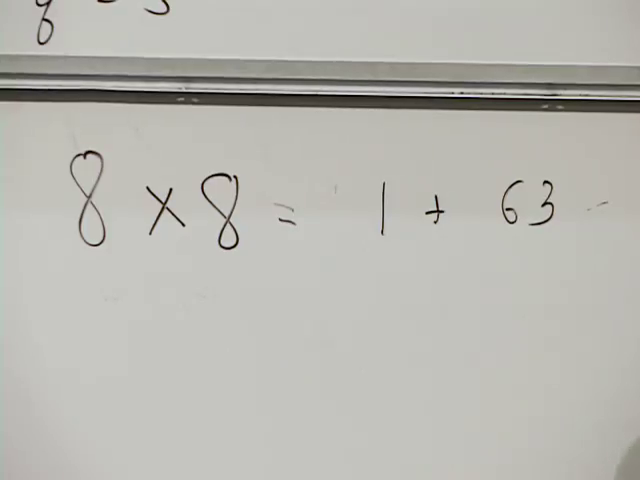
\includegraphics[width=0.68\textwidth]{lecture_04_figure_05.png}\caption{두 글루온 상태의 개수: 64개 상태 가운데 단일항 하나.}\lectureframe{00:53:44}\end{figure}

기약 표현으로 완전히 분해하면 다음과 같습니다.
\begin{equation}
\boldsymbol 8\otimes\boldsymbol 8
=\boldsymbol 1\oplus\boldsymbol 8_S\oplus\boldsymbol 8_A
\oplus\boldsymbol{10}\oplus\overline{\boldsymbol{10}}
\oplus\boldsymbol{27}.
\label{eq:l4-eight-times-eight}
\end{equation}
차원의 합은 다음과 같이 맞습니다.
\begin{equation}
1+8+8+10+10+27=64.
\end{equation}
두 팔중항은 서로 다른 불변 부분 공간입니다. 하나는 수반 표현 인자 두 개의 교환에 대해 대칭이고, 다른 하나는 반대칭입니다. 단일항은 글루볼 상태를 만들 수 있는 두 글루온 색 채널입니다.
\editorialnote{칠판에서는 먼저 \(8\times8=1+63\)만 제시됩니다. 뒤이은 수업 중 문답에서 열거된 기약 차원이 나옵니다. 막대와 대칭성 표기는 표준 \(SU(3)\) 표기법에 맞춰 복원했습니다.}

\subsection{관측되는 전하가 정수인 이유}

쿼크 전하에는 두 종류가 있습니다.
\begin{equation}
Q_{\mathrm{up\text{-}like}}=+\frac23,
\qquad
Q_{\mathrm{down\text{-}like}}=-\frac13.
\end{equation}
따라서 쿼크 세 개의 총전하는 정수입니다. 업형 쿼크가 몇 개인지에 따라 \(-1,0,+1,\text{ or }+2\)가 됩니다. 쿼크와 반쿼크의 전하도 마찬가지로 \(0\) 또는 \(\pm1\)입니다. 글루온은 전기 전하를 띠지 않습니다. 따라서 관측된 쿼크 표현으로 만든 기본 색 단일항은 구성 입자의 전하가 분수여도 전기 전하가 정수입니다.

\begin{classroomqa}
\audiencequestion{기묘 쿼크의 전기 전하는 얼마인가요?
\lecturetimestamp{00:56:08}}
\lecturerresponse{다운형 쿼크이므로 전하는 \(-1/3\)입니다. 세 세대에서도 같은 전하 패턴이 반복됩니다. \((u,d)\), \((c,s)\), \((t,b)\)이며, 각 쌍의 전하는 \(+2/3\)와 \(-1/3\)입니다.}
\end{classroomqa}

이 입자 구성에서는 색 단일항 조건과 전기 전하의 정수성이 밀접하게 연결되어 있지만, 수학적으로 같은 명제는 아닙니다. 전하가 정수라는 결론에는 방금 제시한 특정 표준모형 전하 배정도 필요합니다.

\begin{classroomqa}
\audiencequestion{색 단일항은 얽힌 상태인가요? 그렇다면 벨 실험의 얽힌 쌍과 같은 의미가 있나요?
\lecturetimestamp{00:56:58}}
\lecturerresponse{단일항 색 파동함수는 분명 얽혀 있습니다. 각 색이 따로 확정된 곱상태가 아니라 결맞은 중첩 상태입니다. 원칙적으로 구성 입자들을 서로 떼어 놓을 수는 있지만, 가둠 때문에 분리에 드는 비용은 점점 커지고 결국 새로운 강입자가 만들어집니다. 그러므로 상태는 얽혀 있지만 벨 실험 방식으로 조작하기에는 적합한 계가 아닙니다.}
\end{classroomqa}

\section{텐서곱 방정식의 의미}

이제 곱셈표를 좀 더 구체적으로 설명할 필요가 있습니다. \(\psi_i\)와 \(\phi_j\)를 스핀 1/2인 두 대상을 생성하는 연산자라고 합시다. 전자와 양성자처럼 서로 다른 종을 나타낼 수도 있고, 적절한 통계성을 고려한 같은 종의 두 복사본을 나타낼 수도 있습니다. 각 지표는 두 값을 취합니다. 네 가지 곱
\begin{equation}
\psi_\uparrow\phi_\uparrow,
\quad
\psi_\uparrow\phi_\downarrow,
\quad
\psi_\downarrow\phi_\uparrow,
\quad
\psi_\downarrow\phi_\downarrow
\end{equation}
이 텐서곱 공간을 생성합니다.

군 원소가 각 인자에 \(U\)로 작용한다면, 곱에 대해서는 \(U\otimes U\)로 작용합니다. 성분으로 쓰면
\begin{equation}
\psi_i\phi_j
\longmapsto
U_i{}^kU_j{}^\ell\psi_k\phi_\ell.
\label{eq:l4-product-action}
\end{equation}
이 표현은 4차원이지만 가약 표현입니다. 반대칭 조합
\begin{equation}
\frac{1}{\sqrt2}
(\psi_\uparrow\phi_\downarrow
-\psi_\downarrow\phi_\uparrow)
\end{equation}
은 자기 자신으로 사상되는 반면, 대칭인 세 조합은 서로 사이에서 사상됩니다. 이 조합에 맞는 기저에서는 모든 곱 표현 행렬이 다음과 같은 블록 대각 형태를 띱니다.
\begin{equation}
D_{2\otimes2}(g)
\sim
\begin{pmatrix}
1&0\\
0&D_3(g)
\end{pmatrix}.
\label{eq:l4-spin-block-diagonal}
\end{equation}

\begin{classroomqa}
\audiencequestion{\(\boldsymbol 3\otimes\boldsymbol 3=\bar{\boldsymbol 3}\oplus\boldsymbol 6\)와 같은 방정식은 어떤 연산을 나타내나요?
\lecturetimestamp{00:57:51}}
\lecturerresponse{좌변은 합성 상태 공간을 이룹니다. 군은 두 인자 모두에 작용하므로 곱 기저 상태들을 섞습니다. 우변은 기저를 바꾸면 상태들이 불변 집합으로 나뉜다는 뜻입니다. 세 반대칭 조합은 반삼중항처럼 변환하고, 여섯 대칭 조합은 육중항처럼 변환합니다. 더하기 기호는 보통의 수치 덧셈이 아니라 직합을 뜻합니다.}
\end{classroomqa}

\begin{classroomqa}
\audiencequestion{아홉 상태가 \(3+6\), 또는 \(1+8\)로 분해된다는 것은 어떻게 알 수 있나요? 예를 들어 \(2+7\)일 수도 있지 않나요?
\lecturetimestamp{01:04:39}}
\lecturerresponse{차원만 세어서는 분해를 결정할 수 없습니다. \(SU(3)\)이 어떤 기약 표현을 갖는지 알아야 하고, 지표를 대칭화하거나 반대칭화하거나 자취 부분과 자취 없는 부분을 분리하는 등 불변 부분 공간을 구성해야 합니다. 완전한 분류에는 더 많은 군론이 필요합니다. 여기서는 쿼크와 글루온에 필요한 표현만 사용합니다.}
\end{classroomqa}

불변 엡실론 텐서를 쓰면 단일항 구성이 명확해집니다. \(SU(2)\)에 대해
\begin{equation}
\epsilon_{ij}U^i{}_kU^j{}_\ell
=(\det U)\epsilon_{k\ell}
=\epsilon_{k\ell}.
\end{equation}
따라서 \(\epsilon_{ij}\psi^i\phi^j\)는 불변입니다. \(SU(3)\)에서는 세 지표를 가진 버전으로 다음을 얻습니다.
\begin{equation}
\epsilon_{ijk}U^i{}_aU^j{}_bU^k{}_c
=(\det U)\epsilon_{abc}
=\epsilon_{abc},
\end{equation}
이는 식~\eqref{eq:l4-baryon-singlet}의 쿼크 세 개 상태가 불변임을 증명합니다.

\begin{classroomqa}
\audiencequestion{단일항이 변환되지 않는 이유를 명시적으로 보일 수 있나요?
\lecturetimestamp{01:07:18}}
\lecturerresponse{네. 모든 기본 지표를 완전 반대칭 엡실론 텐서와 수축하면 됩니다. 변환 아래에서는 행렬들의 곱이 엡실론에 \(\det U\)를 곱합니다. 특수 유니터리 행렬의 행렬식은 1이므로 수축한 상태는 변하지 않습니다. \(SU(2)\)에서는 이것이 두 스핀 단일항을 증명하고, \(SU(3)\)에서는 빨강--초록--파랑 쿼크 세 개의 단일항을 증명합니다.}
\end{classroomqa}

\begin{classroomqa}
\audiencequestion{글루온 팔중항 두 개의 완전한 분해는 무엇인가요?
\lecturetimestamp{01:09:24}}
\lecturerresponse{식~\eqref{eq:l4-eight-times-eight}에 나온 분해입니다. 단일항 하나, 팔중항 두 개, 십중항 하나, 반십중항 하나, 그리고 27차원 표현 하나입니다. 팔중항 지표 두 개로 만들 수 있는 색 단일항 조합은 정확히 하나입니다.}
\end{classroomqa}

\begin{classroomqa}
\audiencequestion{쿼크 세 개의 완전한 분해는 이에 대응해 어떻게 되나요?
\lecturetimestamp{01:11:51}}
\lecturerresponse{물리적으로 핵심적인 답은 단일항이 하나 포함된다는 것입니다. 차원 계산까지 완성하면 식~\eqref{eq:l4-three-quark-full}을 얻습니다. 단일항 하나, 팔중항 두 개, 십중항 하나이며 전체 상태 수는 \(1+8+8+10=27\)입니다.\editorialnote{문답 중 강의자는 완전한 \(3\otimes3\otimes3\) 분해를 기억하지 못합니다. 여기에는 표준적인 완성 결과를 명시적으로 보충하고, 이를 구두 답변에 귀속시키지 않았습니다.}}
\end{classroomqa}

같은 생각을 두 글루온 공간으로 확장할 수 있다. 순진한 곱 기저에서는
\(SU(3)\)가 \(64\times64\) 행렬로 작용한다. 기약 성분에 맞춘 기저에서는 이 행렬들이 블록 대각 형태가 된다.
\begin{equation}
\begin{aligned}
D_{8\otimes8}(g)
&\sim
\operatorname{diag}\bigl(
1,D_{8_S}(g),D_{8_A}(g),
\\
&\hspace{4.8em}
D_{10}(g),D_{\overline{10}}(g),D_{27}(g)
\bigr).
\end{aligned}
\end{equation}
어느 블록도 다른 블록과 섞이지 않지만, 각 블록 안의 상태들은 서로 섞인다.

\begin{classroomqa}
\audiencequestion{텐서곱 분해란 큰 표현 행렬이 블록 대각 형태가 되는 기저로 바꾸는 것뿐인가요?
\lecturetimestamp{01:12:02}}
\lecturerresponse{맞습니다. 두 스핀의 경우 4차원 행렬이 1차원 단일항 블록과 3차원 삼중항 블록으로 바뀝니다. 두 글루온의 경우 64차원 행렬이 차원이 \(1,8,8,10,10,\text{ and }27\)인 블록들로 바뀝니다. 각 블록은 모든 군 변환 아래에서 닫혀 있습니다.}
\end{classroomqa}

\begin{classroomqa}
\audiencequestion{전체 텐서곱 공간 안의 그런 닫힌 부분을 부르는 이름이 있나요?
\lecturetimestamp{01:14:55}}
\lecturerresponse{그것은 부분표현을 이루는 불변 부분공간입니다. 더 이상 분해할 수 없으면 기약 표현, 즉 irrep을 이룹니다. 전체 텐서곱은 그런 기약 성분들의 직합입니다.\editorialnote{강의 중에는 질문에서 요청한 용어가 나오지 않는다. 답변에서는 표준 표현론 용어를 제시한다.}}
\end{classroomqa}

\begin{classroomqa}
\audiencequestion{비단일항인 십중항과 다른 표현들을 존재하지 않는다고 부를 때, 완전히 무시해야 한다는 뜻인가요?
\lecturetimestamp{01:15:36}}
\lecturerresponse{그 표현들은 타당한 색 섹터이며 중간 계산에서 중요하지만, 실험실에서 고립된 유한 에너지 입자로 나타나지는 않습니다. 자유 점근 상태가 되지 못하게 하는 것은 표현론의 실패가 아니라 색 가둠입니다.}
\end{classroomqa}

\section{남부의 색 개념에서 색 가둠까지}

색 개념은 QCD의 최종 정식화보다 앞서 나왔다. 요이치로 남부는 이미 1960년대 초에 숨겨진 세 가지 값의 양자수가 눈에 띄는 문제를 해결할 수 있음을 이해했다. 쿼크는 분수 전하를 띠지만, 분수 전하를 가진 자유 입자는 관측되지 않는다는 문제였다. 물리적 상태가 색 단일항으로 제한되면 쿼크는 앞서 설명한 정수 전하 조합으로 나타난다. 남은 문제는 동역학적이다. 유한 에너지 자유 상태가 모두 단일항이 되도록 하는 힘은 무엇인가?

전자기학의 비유부터 살펴보자. 전하와 반대 부호의 전하는 서로 끌어당긴다. 둘을 가까이 가져가면 에너지가 낮아지고, 같은 부호의 전하를 가까이 밀어 붙이려면 일이 필요하다. 장 자체에는 양의 에너지가 저장된다.
\begin{equation}
E_{\mathrm{field}}
=\frac12\int d^3x\,\boldsymbol E^2
\end{equation}
단순한 정전기 단위계에서 성립하는 식이다. 순전하가 있으면 장이 계 바깥 먼 곳까지 뻗어나가지만, 단단히 결합한 중성 쌍에는 근거리 쌍극자 장만 남는다. 따라서 중성화하면 바깥쪽 장 에너지가 사라진다.

전자기 결합을 엄청나게 키운다고 상상해 보자. 순전하에 따른 장 에너지 페널티가 매우 커져 낮은 에너지의 물체는 압도적으로 중성이 되고, 하전된 구성 성분을 떼어내는 비용은 감당하기 어려울 만큼 커질 수 있다. 남부는 이 직관을 색에 적용했다. 여덟 색 전하는 여덟 글루온 장의 원천이므로, 큰 색 장 에너지가 고립된 비단일항 상태를 금지할 수 있다는 생각이었다.

이 직관은 대체로 옳지만, QCD에는 결정적인 새로운 특징이 있다. 광자는 전하를 띠지 않지만 글루온은 색을 띤다. 광자는 고전 전자기장의 원천이 아니며, 맥스웰 방정식은 선형이므로 전자기파 두 개는 중첩되어 서로 통과한다. 글루온은 색 팔중항으로 변환되므로 글루온은 다른 글루온의 원천이 되고 서로 상호작용한다. 하나의 글루온 장 안에서 서로 다른 부분들도 상호작용한다. 따라서 비가환 게이지 장은 비선형이다.

\subsection{플럭스 튜브와 선형 퍼텐셜}

장거리에서 글루온의 자기상호작용은 색 플럭스가 보통의 전기 쌍극자 장처럼 퍼져 나가는 것을 막는다. 플럭스는 쿼크와 반쿼크를 잇는 튜브 안으로 압축된다. 긴 튜브의 장 세기와 단면적은 대략 일정하므로, 튜브에는 길이당 에너지가 대략 일정하게 저장된다. \(\sigma\)를 이 끈 장력이라고 하면,
\begin{equation}
V(R)\simeq\sigma R+\text{constant}
\qquad (R\ \text{large}).
\label{eq:l4-linear-potential}
\end{equation}

\begin{figure}[htbp]
\centering
\includegraphics[width=0.78\textwidth]{lecture_04_figure_06.png}
\caption{쿼크와 반쿼크 사이의 긴 튜브 안에 모인 색 플럭스.}
\lectureframe{01:31:35}
\end{figure}

이는 크기가 \(1/R\)처럼 감소하는 쿨롱 퍼텐셜보다 더 강한 효과다. 색 전하들을 더 멀리 떨어뜨려도 힘이 끝없이 약해지지 않는다. 튜브가 길어지면서 에너지가 계속 더해진다. 무한한 부피 안의 고립된 색 전하에는 끝없이 뻗는 튜브가 필요하므로 에너지가 무한히 커진다. 색 단일항만 유한 에너지 점근 상태를 이룬다는 말의 실제 의미가 바로 이것이다.
\editorialnote{끈 장력 표기와 장거리 퍼텐셜을 명시하여, 균일한 플럭스 튜브가 길이당 균일한 에너지를 가진다는 원문의 설명을 정량적으로 나타낸다.}

\subsection{끈 끊어짐과 제트}

메손 안의 쿼크 하나가 고에너지 충돌을 받는다고 하자. 쿼크가 멀어지기 시작하면 플럭스 튜브가 뒤에서 늘어난다. 쿼크는 운동 에너지를 잃고 다시 끌려올 수 있다. 더 흔하게는 저장된 장 에너지가 충분히 커지면 진공에서 새 쿼크--반쿼크 쌍이 생성된다. 새 반쿼크는 멀어지는 쿼크에 연결된 플럭스를 끝내고, 새 쿼크는 원래 반쿼크에 연결된 플럭스를 끝낸다. 늘어난 단일항 하나가 더 짧은 단일항 둘로 바뀐다.
\begin{equation}
(q\bar q)_{\mathrm{stretched}}
\longrightarrow
(q\bar q)+(q\bar q).
\label{eq:l4-string-breaking}
\end{equation}

\begin{figure}[htbp]
\centering
\includegraphics[width=0.78\textwidth]{lecture_04_figure_07.png}
\caption{쌍 생성은 늘어난 플럭스 튜브 하나를 색 단일항 튜브 두 개로 분리한다.}
\lectureframe{01:34:52}
\end{figure}

\begin{classroomqa}
\audiencequestion{충돌로 튕겨 나온 쿼크가 튜브를 계속 늘릴 만큼 충분한 에너지를 지녔다면, 다시 끌려오는 것 외에 어떤 일이 일어날 수 있나요?
\lecturetimestamp{01:33:50}}
\lecturerresponse{튜브는 쿼크--반쿼크 쌍 생성으로 끊어질 수 있습니다. 튜브의 에너지는 새 쌍의 질량과 운동 에너지가 됩니다. 양 끝이 다시 연결되어 단일항 둘을 이루므로, 이 과정은 고립된 쿼크가 아니라 추가 메손을 생성합니다.}
\end{classroomqa}

그 파톤들 가운데 하나가 여전히 큰 운동량을 지니면 과정이 반복된다. 그 결과 원래 파톤의 진행 방향 주위로 집중된 색 단일항 하드론의 연쇄가 만들어진다. 이를 제트라고 한다. 에너지가 큰 쿼크와 글루온이 하드론으로 바뀌는 과정을 하드론화라고 한다. 제트를 통해 처음 생성된 색 전하 입자를 추론할 수는 있지만, 그 입자 자체가 관측되는 것은 아니다.

\begin{classroomqa}
\audiencequestion{끈 끊어짐으로 메손만 만들어지나요, 아니면 제트에서 다른 하드론도 나올 수 있나요?
\lecturetimestamp{01:35:20}}
\lecturerresponse{물론 다른 하드론도 나올 수 있습니다. 최종적으로 관측되는 물체가 단일항이면 된다는 것이 색에 관한 유일한 조건입니다. 한 번 끊어지는 경우에는 메손이 가장 간단한 그림이지만, 바리온과 반바리온, 더 복잡한 단일항 조합도 생성될 수 있습니다.}
\end{classroomqa}

쿼크 세 개는 색 단일항 접합부에서 플럭스를 끝낼 수 있다. 세 갈래로 뻗는 이 그림은 식~\eqref{eq:l4-baryon-singlet}의 반대칭 엡실론 텐서에 대응하는 동역학적 그림이다. 완전한 바리온에서는 순 색 플럭스가 바깥으로 빠져나오지 않는다.

\begin{figure}[htbp]
\centering
\includegraphics[width=0.72\textwidth]{lecture_04_figure_08.png}
\caption{메손의 끈 끊어짐 그림 아래에 나타낸 바리온의 세 갈래 색 플럭스 접합부.}
\lectureframe{01:36:12}
\end{figure}

\section{게이지 장, 보존 전하와 표준모형}

현재 수준에서 게이지 이론은 보존 전하가 광자와 비슷한 장의 원천이 되는 이론으로 이해할 수 있다. 전하는 전자기장의 원천이고, 여덟 색 전하는 여덟 글루온 장의 원천이다. 더 깊은 정식화에서는 대칭을 국소화하고, 이웃한 시공간 점에서 내부 상태를 비교하는 접속을 도입한다. 그러나 여기서 다루는 색 가둠의 그림에는 그런 구성이 필요하지 않다.
\editorialnote{게이지 이론의 더 깊은 표준적 의미는 국소 대칭을 정식화하는 것으로, 원문에서도 언급만 하고 뒤로 미뤄 둔다.}

대칭, 보존 전하와 플럭스는 긴밀히 연결되어 있다. 장선이 전하에서만 끝날 수 있다면, 원천은 플럭스가 아무것에도 연결되지 않은 채 남도록 그냥 사라질 수 없다. 또한 장의 변화는 인과적으로 전파되므로 그 원천의 먼 곳에 있는 장이 모두 순간적으로 사라질 수도 없다. 국소적인 형태로 같은 물리는 연속 방정식으로 표현된다.
\begin{equation}
\frac{\partial\rho}{\partial t}
+\boldsymbol\nabla\cdot\boldsymbol j=0,
\end{equation}
이 식은 전하가 경계를 통과해 흐를 때만 한 영역 밖으로 나갈 수 있음을 뜻한다. 장선에 관한 논증은 이 국소 보존 법칙을 기하학적으로 그린 것이다.

이제 표준모형 안에서 이 결과가 어디에 놓이는지 살펴볼 수 있다. 색 섹터에는 \(SU(3)\)의 생성원 여덟 개와 이에 대응하는 글루온 장 여덟 개가 있다. 아벨 섹터에는 생성원 하나와 게이지 장 하나가 있다. 생성원 세 개는 보통의 공간 각운동량이 아니라 추가적인 \(SU(2)\)에 속한다. 대칭 깨짐 전 게이지 구조는 다음과 같다.
\begin{equation}
SU(3)_c\times SU(2)_L\times U(1)_Y,
\end{equation}
생성원은 모두 \(8+3+1=12\)개다. 다음으로 전약 \(SU(2)\)을 이해한 뒤, 힉스 장과 관측되는 광자, \(W^\pm\), \(Z\)가 어떻게 나타나는지 살펴보자.
\editorialnote{원문은 광자를 여덟 글루온과 함께 세고, 나머지 인자를 \(SU(2)\times U(1)\)라고 설명한다. 깨지지 않은 표준모형에서 아벨 인자는 초전하 \(U(1)_Y\)이다. 광자는 전약 혼합 뒤에야 나타난다.}

이제 핵심 논리의 연결이 완성되었다. 추상군은 표현을 통해 작용하고, 무한소 생성원은 보존 전하이며, 쿼크와 반쿼크, 글루온은 각각 \(\boldsymbol 3\), \(\bar{\boldsymbol 3}\), \(\boldsymbol 8\) 표현에 속한다. 텐서곱은 단일항 하드론을 식별하고, 비선형 글루온 장은 단일항 선택을 색 가둠이라는 물리적 현상으로 만든다.
